% ═════════════════════════════════════════════════════════════════════════════
% CHAPTER: Results and Evaluation
% ═════════════════════════════════════════════════════════════════════════════

\chapter{Validation, Testing and Results}
\label{chap:results}

% ═════════════════════════════════════════════════════════════════════════════
\section{\textcolor[HTML]{0066CC}{Validation Scope and Approach}}
% ═════════════════════════════════════════════════════════════════════════════

In this chapter we demonstrate the validation approach which was maintained on the LEON prototype once implementation phase was achieved. Our goal is not to state a production deployment but to demonstrate how the services which was implemented were tested and what was really measured during all tests and how these measured enable to reach objectives of the project.

This prototype was largely tested in the \textbf{Copilot Studio test pane}, which serves as the execution test part for the conversational layer. When the test pane is run, the dialogue flow is triggered through the Copilot Studio interface, and through Power Automate business logic is implemented to pull data from the SharePoint/Excel data stores in the same way it was defined in Chapter~\ref{chap:implementation}. The final end user channel will be \textbf{Teams / Microsoft 365 Copilot}, but only the prototype level test is reported at this chapter, assuming the final channel has not yet been deployed to production.

The validation was then carried out along 3 orthogonal axes : the nominal functional use cases were executed for each of the main services, the error conditions were checked, to make sure LEON will favor clarification, graceful fallback or denial instead of failure in silent mode, the access-controlled operations were browsed, from a RBAC point of view, especially regarding read/write on the governance data. To illustrate, if asked “Who owns the External mirrors in J4U?”, it should answer from the Excel file containing the information”, instead of providing a textual free format output. Or, if asked for the gate of a certain component which has no recorded port, since no catalogue entry was created for it, simply says that it diesn't exist in the recorded gate informations.

At this stage, the chapter makes no quantitative claims which have not been formally calculated. There are no numbers, for latency, the number of requests, or the number of statistical errors. The validation is done through scenarios end-to-end(user query $\rightarrow$ workflow execution $\rightarrow$ data access $\rightarrow$ response), with execution traces (e.g. workflow run history) and typical error handling examples.
% ═════════════════════════════════════════════════════════════════════════════
\section{\textcolor[HTML]{0066CC}{Functional Test Scenarios}}
% ═════════════════════════════════════════════════════════════════════════════

The functional campaign is based on some typical users requests that can be grouped to the basic services implemented in LEON. Table~\ref{tab:functional-validation-scenarios} summarizes some typical scenarios, their preconditions and their resulting behavior on the prototype.

\begin{table}[H]
\centering
\footnotesize
\renewcommand{\arraystretch}{1.25}
\caption{Representative functional test scenarios used for LEON prototype validation.}
\label{tab:functional-validation-scenarios}
\begin{tabularx}{\textwidth}{|p{0.9cm}|p{2.9cm}|p{2.6cm}|X|X|p{1.8cm}|}
\hline
\rowcolor[HTML]{E6F2FF}\textcolor[HTML]{003D99}{\textbf{ID}} & \textcolor[HTML]{003D99}{\textbf{User request}} & \textcolor[HTML]{003D99}{\textbf{Preconditions}} & \textcolor[HTML]{003D99}{\textbf{Expected result}} & \textcolor[HTML]{003D99}{\textbf{Obtained result}} & \textcolor[HTML]{003D99}{\textbf{Status}} \\
\hline
FT-01 & ``Who is responsible for Brake System in J4U?'' & The project sheet can be found within the Who-is-Who workbook, the component line and role column are carried out. & LEON recognizes project sheet and computes component/role pair and return the responsible person from Excel. & In the prototype path the conversational answer is transmitted following that the Excel source and the governance owner have read from the work book structure Figure~\ref{fig:w1-dataset-structure}. & Validated \\
\hline
FT-02 & ``What is the current gate for Suspension System in J4U?'' & The gate repositories are located in SharePoint; there are a lot of components stored within gates in SharePoint. & LEON will read through the recorded gate repositories and report the highest gate achieved by the component. & The reply we get depends on whether there are files present in gate folders ,see lookup logic Figure~\ref{fig:gate-detection-workflow}. & Validated \\
\hline
FT-03 & ``Update the DRE for External mirrors in J4U to John Doe.'' & User has permission to change the source workbook; project, component and role can be resolved. & LEON sends a confirmation request, the target cells will then be configured in Power Automate and an explicit message is sent back for confirmation. & The prototype flow illustrates the step through a clean update and concludes with a message that the write operation as demonstrated in Figures~\ref{fig:update-execution} and ~\ref{fig:update-write}. & Validated \\
\hline
FT-04 & ``Send a reminder to the responsible engineer for Brake System.'' & Recipient can be looked up from directory data; available subject/body or template data available. & The LEON resolves the recipient, create the message payload, send the notification/ draft path without exiting the conversational flow. & The prototype behavior we will focus on is the email capture and recipient resolution path illustrated in Figure~\ref{fig:email-assistant-flow}. & Validated \\
\hline
FT-05 & ``Validate this specification against the configured rules.'' & SpecValidator possesses a specification document and a collection of related rules. & Validator runs in a non-mutable and deterministic way and produce a structure of validation result. & The prototype was designed to enable a defined execution of rules and the production of a report. & Partially documented \\
\hline
\end{tabularx}
\end{table}

The selected scenarios reflect the primary value offered to the end-users of the prototype: access information on governance, read project maturity using documented evidence, amend the controlled information, send context aware communication and check the specifications using deterministic rules.\\
\noindent\textbf{Confidentiality note.} All screen captures contained within this chapter are disguised examples. All names, e-mail accounts, internal ids, share point URLs, housing paths will need to be obscured for the jury copy.

\begingroup
\setlength{\intextsep}{6pt}
\setlength{\textfloatsep}{6pt}
\setlength{\floatsep}{6pt}
\captionsetup[figure]{skip=4pt}

\subsection{\textcolor[HTML]{003D99}{Who-is-Who Scenario Evidence}}

The Who-is-Who test sequence was tested in a live lookup path: user requests the name of a responsible on a specific project and component, and the conversational layer identifies the project context and the backend logic to route the request to the governance dataset. The actual feasibility of this scenario depends on two observable aspects: the assistance being aware of the name of the project entered by the user and the orchestration managing the lookup or redirect when the expected record does not exist.
\begin{figure}[H]
\centering
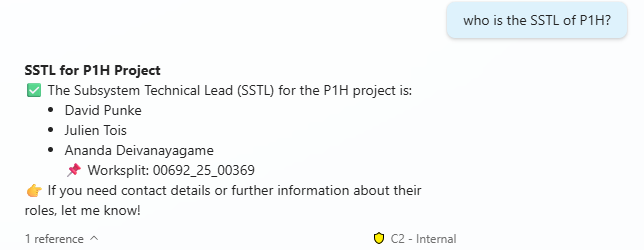
\includegraphics[width=0.8\textwidth]{images_pfe/who is who1.png}
\caption{Anonymized Copilot Studio capture used to support project disambiguation during the Who-is-Who validation path.}
\label{fig:results-who-conversation}
\end{figure}

\subsection{\textcolor[HTML]{003D99}{Gate Status Scenario Evidence}}

For gate status retrieval, the evidence needed to support the argument that the assistant searches through documents as opposed guessing at runtime via conversational utterance. Copilot Studio knowledge configuration is used for gate reasoning as a visual evidence, and the gate interpretation rule as an other visual evidence for highest documented maturity level return.


\subsection{\textcolor[HTML]{003D99}{Responsible Update Scenario Evidence}}

The update case is the most sensitive function path because it combines user input, authorization, write, and confirmation. The first proof here is regarding to conversation input state where user supply the real component fragment to go on the update procedure. The second proof shows the backend action‘s signature in order to supply update parameters to flow.



\subsection{\textcolor[HTML]{003D99}{Email and Notification Scenario Evidence}}

The use case was proved with the help of request path where LEON receives necessary inputs from the user intent, determines the recipient through directory connector, prepares delivery for the action message. Critical issues highlighted are on controlled execution such as before completing the input values it should not be delivering a notification.

\begin{figure}[H]
\centering
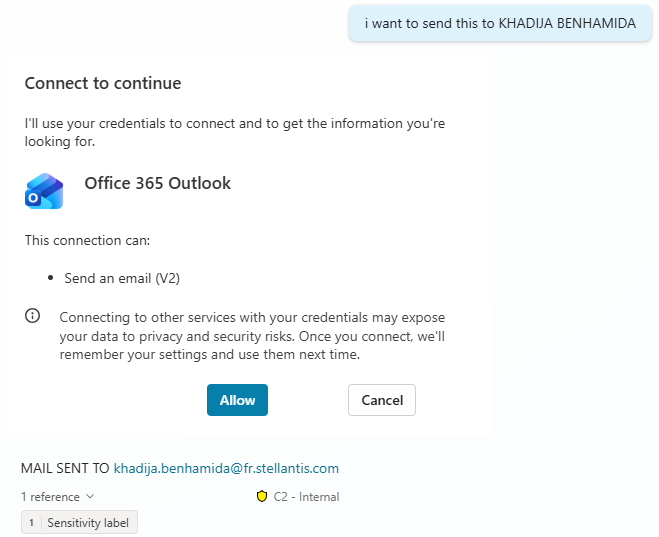
\includegraphics[width=0.72\textwidth]{images_pfe/email1.png}
\caption{Anonymized conversational capture used during e-mail and notification validation for request capture and field completion.}
\label{fig:results-email-conversation}
\end{figure}

\begin{figure}[H]
\centering
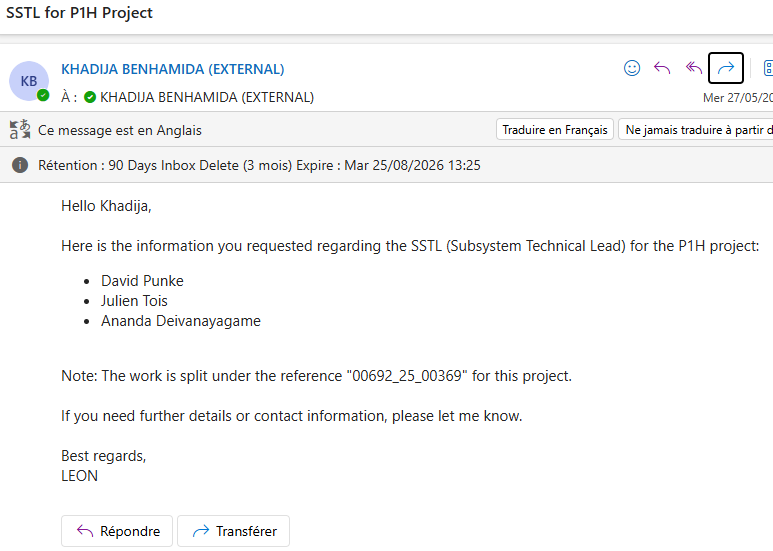
\includegraphics[width=0.42\textwidth]{images_pfe/email2.png}
\caption{Anonymized backend connector capture showing the notification path through recipient lookup and e-mail sending actions.}
\label{fig:results-email-flow}
\end{figure}
\begin{figure}[H]
\centering
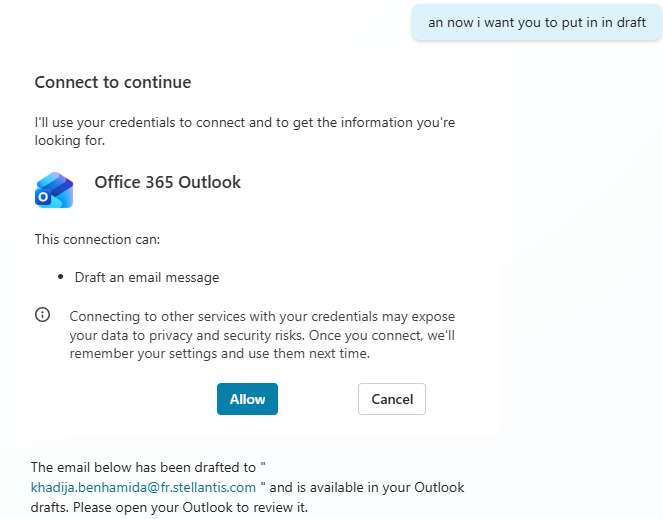
\includegraphics[width=0.72\textwidth]{images_pfe/email3.png}
\caption{Anonymized conversational capture used during e-mail and notification validation for request capture and field completion.}
\label{fig:results-email-conversation}
\end{figure}

\begin{figure}[H]
\centering
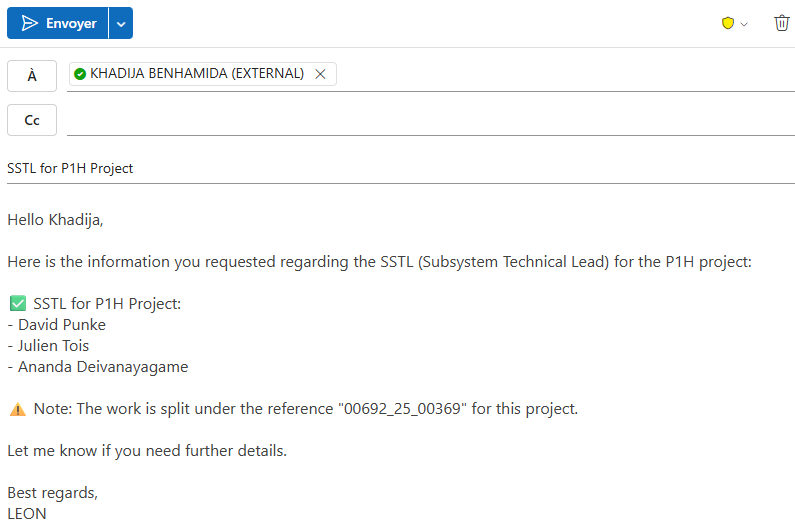
\includegraphics[width=0.42\textwidth]{images_pfe/email4.png}
\caption{Anonymized backend connector capture showing the notification path through recipient lookup and e-mail sending actions.}
\label{fig:results-email-flow}
\end{figure}
\subsection{\textcolor[HTML]{003D99}{SpecValidator Scenario Evidence}}

The SpecValidator path is less conversational than the governance services, but it still begins from the same prototype entry point. In the current working set of screenshots, the available evidence shows the test environment used to launch the scenario and the validation backend that executes deterministic checks. A dedicated anonymized test-pane capture of the exact validation request would remain preferable in a final defended version.



% ═════════════════════════════════════════════════════════════════════════════
\section{\textcolor[HTML]{0066CC}{Error and Robustness Testing}}
% ═════════════════════════════════════════════════════════════════════════════

It appeared that a nominal execution with general nominality execution was insufficient for a governance assistant. In fact, in real execution, the prototype also had to manage implicit cases where the user did not finish his request, or the asked entity or the backend source could be inaccessible. So robustness tests aimed at explicit error paths already modeled in implementation.
\begin{table}[H]
\centering
\footnotesize
\renewcommand{\arraystretch}{1.25}
\caption{Error and robustness scenarios checked during prototype validation.}
\label{tab:robustness-validation-scenarios}
\begin{tabularx}{\textwidth}{|p{3cm}|p{2.7cm}|X|p{2.2cm}|}
\hline
\rowcolor[HTML]{E6F2FF}\textcolor[HTML]{003D99}{\textbf{Error code}} & \textcolor[HTML]{003D99}{\textbf{Typical trigger}} & \textcolor[HTML]{003D99}{\textbf{Expected prototype behavior}} & \textcolor[HTML]{003D99}{\textbf{Control mode}} \\
\hline
\texttt{PROJECT NOT FOUND} & Unknown or misspelled project name & LEON does not quietly guess. It either asks a question or guesses the nearest known project name if there is a reasonable default option. & Clarification \\
\hline
\texttt{COMPONENT NOT FOUND} & Missing component from Excel sheet or file store & LEON interrupts the nominal path and asks user to give a better component name instead of providing an invalid result. & Clarification \\
\hline
\texttt{ROLE NOT FOUND} & The selected project has no specified roles & Indicates that the role is not present in the current context and then suggests available roles. & Clarification \\
\hline
\texttt{UNAUTHORIZED} & User attempts to read/write but lacks inherited privilege & The flow must stop, the backend execution must be visible on the refusal path and  the user must receive a clear authorization message. & Refusal / escalation \\
\hline
\texttt{DATASET UNAVAILABLE} & SharePoint, Excel or any other backend connector is currently down & LEON responds that the request cannot be serviced at the present time and recommends retrying or escalating. & Fallback \\
\hline
\end{tabularx}s
\end{table}

The validation rule remains the same: Any implicit or undeclared situation must be mapped to an explicit control flow on the conversation. For example a non-existing component name would then raise a reformulate request. A permission failure would prevent the action from performing and leave a history mark on the backend execution history.


% ═════════════════════════════════════════════════════════════════════════════
\section{\textcolor[HTML]{0066CC}{Security Validation and RBAC Review}}
% ═════════════════════════════════════════════════════════════════════════════

The review of RBAC was not made by non specified implicit internal rules but by testable empirical behaviors of the system. With LEON, there is no re-definition of the enterprise permissions: they are inherited from the access rights for the linked repository or connectors. This is an important aspect for governance, as the same conversational query can result in read success, write success, and deny based on the access rights on the SharePoint or the Excel sheet.\\

Two types of case are considered in validation: \textbf{authorization} or \textbf{non-authorization} cases. If the case is an authorization, then the request is authorized, the workflow proceeds as expected, and data is read or written. If the case is a non-authorization, then the request will not even reach a hidden workaround. The action is denied and a clear message appears to the user. The execution back-path can be visualized through the “Power Automate” run history. Realistically, someone with write access to a responsibility assignment should see the update process, while someone without it should have the flow blocked by an authorization message rather than a partial, hidden, or invisible modification.\\
The full proof of the this security test is (1) \textbf{the client message stating the permission} is allowed or denied to the end-user and (2) the \textbf{flow trace} proving if Power Automate flowed through the flow or not, and (3) \textbf{the modification side effect} to the source data if it were not to be changed at all. There is enough information to guarantee the RBAC prototype as it prove that we effect on the execution path and not only on the words displayed to the user.
\begin{table}[H]
\centering
\footnotesize
\renewcommand{\arraystretch}{1.25}
\caption{RBAC-oriented comparison between authorized and non-authorized prototype behaviors.}
\label{tab:rbac-validation-cases}
\begin{tabularx}{\textwidth}{|p{2.7cm}|p{2.6cm}|X|X|}
\hline
\rowcolor[HTML]{E6F2FF}\textcolor[HTML]{003D99}{\textbf{Case}} & \textcolor[HTML]{003D99}{\textbf{Example action}} & \textcolor[HTML]{003D99}{\textbf{Expected evidence}} & \textcolor[HTML]{003D99}{\textbf{Observed prototype behavior}} \\
\hline
Authorized & Inherit write permission to update the assignment & The conversational confirmation with the desired outcome the successful completion of a backend path with the expected data change is reflected in source workbook. & Update path finishes and returns success in explicit mode after flow receives the parameters \\
\hline
Non-authorized & Test with the same change that demands authorization to continue & Direct refusal message,  source data remains unchanged. & The guarded branch passes on a failure/refuse path rather than hidden or partial change. \\
\hline
\end{tabularx}
\end{table}


\endgroup

% ═════════════════════════════════════════════════════════════════════════════
\section{\textcolor[HTML]{0066CC}{Results and Technical Observations}}
% ═════════════════════════════════════════════════════════════════════════════

The validation work demonstrate that the prototype is actually executing all the main governance scenarios along an end-to-end chain, starting from the request input in Copilot Studio, moving through the Conversational Topic structure, up to Power Automate execution and resolution with enterprise data source and validation rules.There is no question of performance, it‘s more about the coherence between the user request and the back-end answer.

The below technical notes have been derived from tests and also from reviewing implemented flows:

\begin{itemize}
	\item The better the quality of source repositories, the better the answer will be to the governance questions. Naming inconsistencies between Excel sheets cause difficulty for matches even in the off-branch Whose-is-Who service which has naming normalization and fallback to default source when fails.
	\item The retrieval of gate status should rely on how well documents are organized in the gate repositories. In the case where a deliverable may be missing, in the wrong directory, or not yet available, LEON should assign no evidence to that state of maturity.
	\item Update service is more sensitive than read-only query due to interpretation, authorization, authorization and write execution, therefore, positive acknowledgment and traceability is important even in prototype.
	\item Email/notification functionalities are presented as enterprise features rather than general text-generation. Receiver resolution, quality of message and connector availability of mail box determine whether the request will be delivered to delivery, refinement or rejection.
	\item SpecValidator is the most deterministic of the block in the architecture, because its output is driven by a fixed document of rules applied to a fixed input, and not by the nuances of dialogue, therefore it provides a very suitable method for repeatable checking of compliance, given that the rules are explicitly version controlled, as are the inputs.
\end{itemize}

Based on all the above findings and conclusions, we can see that the prototype is working as expected, but we should still consider as a proved up to prototype, not an industrialized service deliver. The Copilot Studio Test pane is good for a proof of behavior and integration logic, but cannot replace a full operational system on the actual end-user channel.
% ═════════════════════════════════════════════════════════════════════════════
\section{\textcolor[HTML]{0066CC}{Synthesis Against Project Objectives (SO1..SO5)}}
% ═════════════════════════════════════════════════════════════════════════════

The final section of the validation chapter relates back to the sub-objectives defined earlier in this report. Table~\ref{tab:results-vs-objectives} pulls these together without overstating what has, and has not, been demonstrated by prototype.

\begin{table}[H]
\centering
\footnotesize
\renewcommand{\arraystretch}{1.25}
\caption{Synthesis of validation results against project objectives SO1 to SO5.}
\label{tab:results-vs-objectives}
\begin{tabularx}{\textwidth}{|p{2.5cm}|X|p{2.5cm}|}
\hline
\rowcolor[HTML]{E6F2FF}\textcolor[HTML]{003D99}{\textbf{Objective}} & \textcolor[HTML]{003D99}{\textbf{Validation evidence}} & \textcolor[HTML]{003D99}{\textbf{Assessment}} \\
\hline
SO1 -- Who-is-Who Lookup & This target is covered by scenario FT-01 as well as the workbook structure in Figure~\ref{fig:w1-dataset-structure}, lookup path in Figure~\ref{fig:w4-lookup}, and the explicit fallback as in Figure~\ref{fig:w5-error-condition}.  From this it can be seen that the prototype can be enabled to read the responsibility information from the appropriate source of governance and explicitly handle uncaught instances. & Validated at prototype level \\
\hline
SO2 -- Gate Status Support & This concept is clarified through the use of scenario FT-02 as shown in Figure~\ref{fig:gate-knowledge-structure}, detection architecture as shown in Figure~\ref{fig:gate-detection-workflow}, and tests for robustness under cases that are missing or ambiguous, to illustrate that the state of a gate is derived from a documentation based gate repository rather than a prediction. & Validated at prototype level \\
\hline
SO3 -- Document Management Support & The actual implementation show that LEON has already a gate based document organization at the SharePoint level, due to the gate-status scenario. The complete path of document upload is still visible in the implementation chapter, because it was an extension that has not yet been done. Therefore this objective is only partially achieved. & Partially validated \\
\hline
SO4 -- Communication Support & Shows that for FT-04, the email service defined in Figure~\ref{fig:email-architecture}, and the path used to capture conversation and distribute to recipients as described in Figure~\ref{fig:email-assistant-flow}, a messaging service is able to collect message parameters, determine recipients and spread an organized notification path with predefined failure cases. & Validated at prototype level \\
\hline
SO5 -- SpecValidator (Compliance Checking) & FT-05 gives a notion of the method chosen to perform the validation service; a deterministic validation service with the component distinct from the one for the conversational variation, is shown to be the Chapter~\ref{chap:implementation} ,the logic of the architecture is coherent to the one wanted. Nevertheless the specification of the set of validated rule and reference sample corpus ought to be more precise in the report. & Validated in principle, documentation still to be completed \\
\hline
\end{tabularx}
\end{table}

To summarize, this synthesis finally proves that the main functionalities objectives of LEON have been met on a prototype scale specifically relating to governance lookup, gate-status support, wired update flow, and help in communication. However the missing element does not lie with either a dominant design trend of the project but in the relative maturity of some extensions, and the quality of documentation for some validation assets especially the SpecValidator and document upload functionalities. 
% ═════════════════════════════════════════════════════════════════════════════
\section*{Questions to Clarify}
% ═════════════════════════════════════════════════════════════════════════════

\begin{itemize}
	\item Which exact sample specification document and rule set were used to validate the SpecValidator path?
	\item Should SO3 be kept as partially achieved because document upload is still described as in development, or has an end-to-end upload scenario since been validated?
	\item Was the final user channel also exercised in Teams / Microsoft 365 Copilot, or should the chapter explicitly state that validation remained limited to Copilot Studio test pane?
\end{itemize}

